\let\negmedspace\undefined
\let\negthickspace\undefined
\documentclass[journal]{IEEEtran}
\usepackage[a5paper, margin=10mm, onecolumn]{geometry}
%\usepackage{lmodern} % Ensure lmodern is loaded for pdflatex
\usepackage{tfrupee} % Include tfrupee package

\setlength{\headheight}{1cm} % Set the height of the header box
\setlength{\headsep}{0mm}  % Set the distance between the header box and the top of the text

\usepackage{gvv-book}
\usepackage{gvv}
\usepackage{cite}
\usepackage{amsmath,amssymb,amsfonts,amsthm}
\usepackage{algorithmic}
\usepackage{graphicx}
\usepackage{textcomp}
\usepackage{xcolor}
\usepackage{txfonts}
\usepackage{listings}
\usepackage{enumitem}
\usepackage{mathtools}
\usepackage{gensymb}
\usepackage{comment}
\usepackage[breaklinks=true]{hyperref}
\usepackage{tkz-euclide} 
\usepackage{listings}
% \usepackage{gvv}                                        
\def\inputGnumericTable{}                                 
\usepackage[latin1]{inputenc}                                
\usepackage{color}                                            
\usepackage{array}                                            
\usepackage{longtable}                                       
\usepackage{calc}                                             
\usepackage{multirow}                                         
\usepackage{hhline}                                           
\usepackage{ifthen}                                           
\usepackage{lscape}
\begin{document}

\bibliographystyle{IEEEtran}
\vspace{3cm}

\title{9.2.4}
\author{EE24BTECH11015 - Dhawal}

% \maketitle
% \newpage
% \bigskip
{\let\newpage\relax\maketitle}

\renewcommand{\thefigure}{\theenumi}
\renewcommand{\thetable}{\theenumi}
\setlength{\intextsep}{10pt} % Space between text and floats

\textbf{Question:}\\
For the Differential Equation $y^{\prime}=\frac{xy}{1+x^2}$, verify that $y=\sqrt{1+x^2}$ is a solution of the differential equation.

\solution{
Solving the given D.E. , we get,
\begin{align}
    \frac{dy}{dx} &=\frac{xy}{1+x^2} \\
    \implies \frac{dy}{y} &= \frac{x}{1+x^2}dx
\end{align}
Integrating both sides we get,
\begin{align}
    \implies    \int \frac{dy}{y} &= \int \frac{x}{1+x^2}dx\\
    \implies    \int \frac{dy}{y} &= \int \frac{1}{2} \frac{2x}{1+x^2}dx\\
    \implies    \ln{y} &=\frac{1}{2} \ln\brak{1+x^2}\\
    \implies    \ln{y} &= \ln\sqrt{1+x^2}
\end{align}
Taking antilog both sides we get,
\begin{align}
    \implies y &= \sqrt{1+x^2}
\end{align}
Thus, $y=\sqrt{1+x^2}$ is a solution to the differential equation $y^{\prime}=\frac{xy}{1+x^2}$.
}\\
\textbf{Computational Solution:}\\
Using classical defination of derivative we get,\\
\begin{align}
    f^{\prime}\brak{x} &= \frac{f\brak{x+h}-f\brak{x}}{h}\\
    \implies f\brak{x+h} &= f\brak{x} + h f^{\prime}\brak{x}
\end{align}
By increasing $x_n$ each iteration by $h$, we are getting $y$ by 
For,
\begin{align}
x_0 &= 0\\
y_0 &= 1\\
h &= 0.01\\
n &= 500
\end{align}
Using Euler Method, we get difference equation,
\begin{align}
y_{n+1} &= y_n + h\frac{dy}{dx}\Big|_{\brak{x_n,y_n}}\\
	y_{n+1} &= y_n + h \frac{x_n}{\sqrt{1+{x_n}^2}}
\end{align}

\begin{figure}[h]
    \centering
    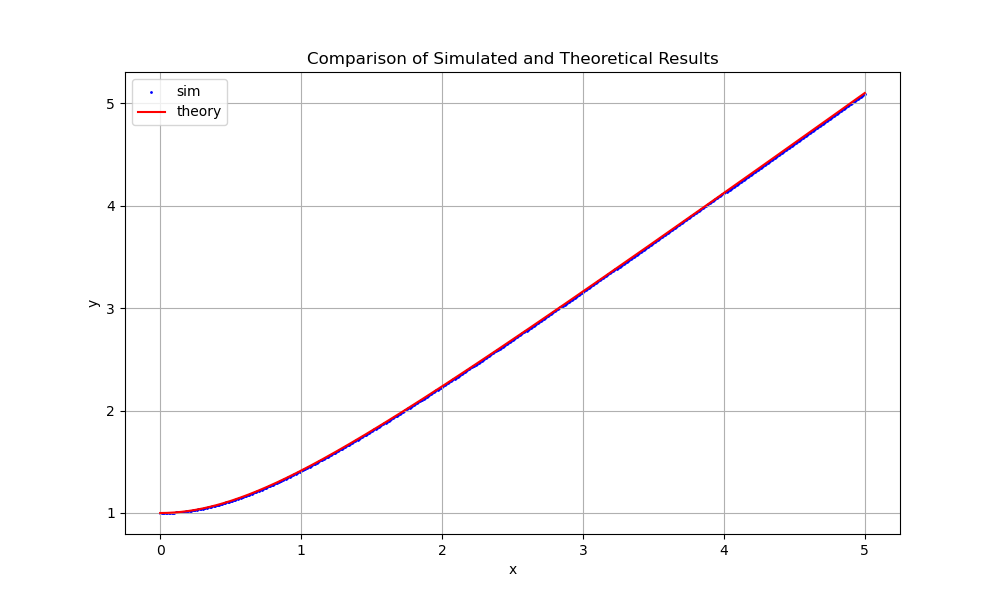
\includegraphics[width=\columnwidth]{figs/Figure_1}
    \caption{Plot of the differential equation }
    \label{fig:Plot}
    \end{figure}

\end{document}
